\documentclass[12pt,landscape]{article}
\usepackage{ling}
\usepackage{multirow}
\usepackage{rotating}
\usepackage[hmargin=2.54cm,vmargin=2.54cm]{geometry}
\geometry{a4paper}
\usepackage{setspace}
\usepackage{booktabs}
\usepackage{array}
\usepackage{colortbl}
\usepackage{tikz}
\usepackage{tikz-qtree}
\usepackage{hhline}
\usepackage{listings}
\PassOptionsToPackage{table}{xcolor}

\usetikzlibrary{arrows,decorations.pathmorphing,backgrounds,positioning,fit,matrix,trees,mindmap,shapes}

\special{papersize=14in,9in}
\setlength{\paperwidth}{14in}
\setlength{\paperheight}{9in}
\setlength{\textwidth}{14in}
\setlength{\textheight}{10in}



\begin{document}


\doublespacing

\includegraphics[scale=.3]{menu.png}

\vspace{-1.65in}
\begin{center}
\hspace{6.5in}
\begin{tabular}{cccccc}
		\hline
		\multicolumn{1}{|c|}{\textbf{+ Silábica}}  & \multicolumn{2}{c|}{}                     & \multicolumn{1}{c|}{} & \multicolumn{2}{c|}{\textbf{-- Anterior}} \\ [-2ex]
		\multicolumn{1}{|c|}{\textbf{+ Resonante}} & \multicolumn{2}{c|}{\phantom{..}\textbf{-- Retraída}\phantom{..}} & \multicolumn{1}{c|}{} & \multicolumn{2}{c|}{\small{(+ redondeada,}} \\ [-2ex]
		\multicolumn{1}{|c|}{\textbf{+ Continua}}  & \multicolumn{2}{c|}{}                     & \multicolumn{1}{c|}{} & \multicolumn{2}{c|}{\small{+ retraída)}} \\
		\hline
		\multicolumn{1}{|c|}{+ Alta}               & \multicolumn{2}{c}{[ i ]}                        & \phantom{thisisfiller} &   & \multicolumn{1}{c|}{[ u ]} \\
		\cline{1-1}
		\multicolumn{1}{|c|}{}                     & \multicolumn{2}{r}{[ e ]\phantom{.}}                        &  & \multicolumn{2}{l|}{\phantom{.}[ o ]}  \\
		\cline{1-1}
		\multicolumn{1}{|c|}{+ Baja}               &                                           &  & [ a ] &   & \multicolumn{1}{c|}{} \\
		\hline
		                     &                                           &  & \multicolumn{1}{|c|}{Deslizadas:} & & \\ [-1ex]
							 &                                           &  & \multicolumn{1}{|c|}{-- silábicas} & & \\
		\cline{4-4}
	\end{tabular}
\end{center}

\begin{center}
\hspace{8in}
	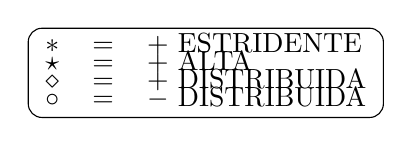
\begin{tikzpicture}
	\node (table) [inner sep=0pt] {
	\begin{tabular}{ccl}
		$\ast$     & = & $+$ ESTRIDENTE \\ [-1.25ex]
		$\star$    & = & $+$ ALTA \\ [-1.25ex]
		$\diamond$ & = & $+$ DISTRIBUIDA \\ [-1.25ex]
		$\circ$    & = & $-$ DISTRIBUIDA \\
	\end{tabular}
	};
	\draw [rounded corners=.5em] (table.north west) rectangle (table.south east);
	\end{tikzpicture}
\end{center}


%\vspace{-1.5in} use this spacing with author names
\vspace{-1.5in}
\begin{center}
%\hspace{-1.5in} use this spacing with author names
\hspace{-1.5in}
\begin{tikzpicture}
	\node (table) [inner sep=0pt] {
	\begin{tabular}{|ll|l|p{1.5cm}|p{1.5cm}|p{1.5cm}|p{1.5cm}|p{1.6cm}|p{1.5cm}|p{1.5cm}|p{1.5cm}|p{1.5cm}|p{1.5cm}|ll|}
\cline{4-13}
\multicolumn{3}{c|}{} & \multicolumn{5}{c|}{\textbf{+ Anterior}} & \multicolumn{5}{c|}{\textbf{-- Anterior}} & \multicolumn{2}{c}{} \\
\cline{4-13}
\multicolumn{3}{c|}{} & \multicolumn{2}{c|}{\textbf{Labial (+ o,u,w)}} & \multicolumn{3}{c|}{\textbf{Coronal}} & \multicolumn{2}{c|}{\textbf{Corono-dorsal}} & \multicolumn{2}{c|}{\textbf{Dorsal}} & \multicolumn{1}{c|}{} \\
\cline{3-13}
\hhline{~~-} \multicolumn{2}{c|}{} & \multicolumn{1}{c|}{\textbf{\cellcolor[gray]{0.75} + Sonora}} & \multirow{2}{*}{\textbf{Bilabial}} & \multirow{2}{*}[1.5mm]{\phantom{..}\textbf{Labio-}} & \multirow{2}{*}[1.5mm]{\phantom{..}\textbf{Inter-}} & \multirow{2}{*}{\phantom{.}\textbf{Dental}} & \multirow{2}{*}{\textbf{Alveolar}} & \multirow{2}{*}[1.5mm]{\phantom{..}\textbf{Alveo-}} & \multirow{2}{*}{\phantom{.}\textbf{Palatal}} & \multirow{2}{*}{\phantom{..}\textbf{}} & \multirow{2}{*}{\phantom{.}\textbf{Uvular}} & \multirow{2}{*}{\phantom{.}\textbf{Glotal}} & \multicolumn{2}{c}{} \\
\cline{3-3}
\hhline{~~-} \multicolumn{2}{c|}{} & \multicolumn{1}{c|}{\textbf{\cellcolor[gray]{0.9}+ Sorda}} & & \multicolumn{1}{c|}{\textbf{dental}} & \multicolumn{1}{c|}{\textbf{dental}} & & & \multicolumn{1}{c|}{\textbf{palatal}} & & & & & \multicolumn{2}{c}{} \\
\cline{3-15}
\hhline{~~-} \multicolumn{2}{c|}{} & \multirow{2}{*}{\phantom{...}\textbf{Oclusivas}} & \multicolumn{1}{c|}{\cellcolor[gray]{0.9} [ p ]} & & & \multicolumn{1}{c|}{\cellcolor[gray]{0.9} [ \textsubbridge{t} ]} & & & & \multicolumn{1}{c|}{\cellcolor[gray]{0.9} [ k ]} & & & & \multirow{4}{*}{\begin{turn}{-90}\phantom{......}\textbf{+ Obstruyente}\end{turn} \phantom{..}} \\
\hhline{~~~----------}
\multicolumn{2}{c|}{} & & \multicolumn{1}{c|}{\cellcolor[gray]{0.75} [ b ]} & & & \multicolumn{1}{c|}{\cellcolor[gray]{0.75} [ \textsubbridge{d} ]} & & & \multicolumn{1}{c|}{\cellcolor[gray]{0.75} [ \textbardotlessj \ ]} & \multicolumn{1}{c|}{\cellcolor[gray]{0.75} [ \textscriptg \ ]} & & & & \\
\hhline{-------------}
\multirow{8}{*}{\begin{sideways}\textbf{+ Continua}\end{sideways}}	 & \multirow{8}{*}{\begin{sideways}(vocales y deslizadas)\end{sideways}} & \multirow{2}{*}{\phantom{...}\textbf{Fricativas}} & \multicolumn{1}{c|}{\cellcolor[gray]{0.9} [ \textphi \ ]} & \multicolumn{1}{c|}{\cellcolor[gray]{0.9} [ f ]} & \multicolumn{1}{c|}{\cellcolor[gray]{0.9} [ \texttheta \ ]} & & \multicolumn{1}{c|}{\cellcolor[gray]{0.9} [ \textinvsubbridge{s} ] [ s ]} & \multicolumn{1}{c|}{\cellcolor[gray]{0.9} [ \textesh \ ]} & & \multicolumn{1}{c|}{\cellcolor[gray]{0.9} [ x ]} & \multicolumn{1}{c|}{\cellcolor[gray]{0.9} [ \textchi \ ]} & \multicolumn{1}{c|}{\cellcolor[gray]{0.9} [ h ]} & & \\
		\hhline{~~~----------}
	 	& & & & & & & \multicolumn{1}{c|}{\cellcolor[gray]{0.75} [ z ]} & \multicolumn{1}{c|}{\cellcolor[gray]{0.75} [ \textyogh \ ]} & \multicolumn{1}{c|}{\cellcolor[gray]{0.75} [ \textctj \ ]} & & & \multicolumn{1}{c|}{\cellcolor[gray]{0.75} [ \texthth \ ]} & & \\
	 	\hhline{~~-----------}
	 	& & \multirow{2}{*}{\phantom{...}\textbf{Africadas}} & & & & & & \multicolumn{1}{c|}{\cellcolor[gray]{0.9} [ \textteshlig \ ]} & & & & & & \\
	 	\hhline{~~~----------}
	 	& & & & & & & & \multicolumn{1}{c|}{\cellcolor[gray]{0.75} [ \textdyoghlig \ ]} & & & & & & \\
	 	\hhline{~~-------------}
	 	& & \multirow{2}{*}{\textbf{Aproximantes}} & & & & & & & & & & & \multirow{5}{*}{\begin{turn}{-90}\hspace{-3mm}(vocales y deslizadas)\end{turn}} & \multirow{5}{*}{\begin{turn}{-90}\hspace{-3mm}\textbf{+ Resonante}\end{turn}} \\
	 	\hhline{~~~----------}
	 	& & & \multicolumn{1}{c|}{\cellcolor[gray]{0.75} [ \textlowering{\textbeta} ]} & & & \multicolumn{1}{c|}{\cellcolor[gray]{0.75} [ \textlowering{\dh} ]} & & & \multicolumn{1}{c|}{\cellcolor[gray]{0.75} [ j ]} & \multicolumn{1}{c|}{\cellcolor[gray]{0.75} [ \textlowering{\textgamma} ] [ w ]} & & & & \\
	 	\hhline{~~-----------}
	 	& & \multirow{2}{*}{\phantom{....}\textbf{Líquidas}} & & & \multicolumn{1}{c|}{\cellcolor[gray]{0.75} [ \textsubbar{l} ]} & \multicolumn{1}{c|}{\cellcolor[gray]{0.75} [ \textsubbridge{l} ]} & \multicolumn{1}{c|}{\cellcolor[gray]{0.75} [ l ]} & \multicolumn{1}{c|}{\cellcolor[gray]{0.75} [ \textrtaill \ ]} & \multicolumn{1}{c|}{\cellcolor[gray]{0.75} [ \textturny \ ]} & & & & & \\
	 	\hhline{~~~----------}
	 	& & & & & & & \multicolumn{1}{c|}{\cellcolor[gray]{0.75} [ \textfishhookr \ ] [ r ]} & & & & \multicolumn{1}{c|}{\cellcolor[gray]{0.75} [ \textscr \ ]} & & & \\
	 	\hhline{-------------}
\multicolumn{2}{c|}{} & \phantom{.....}\textbf{Nasales} & \multicolumn{1}{c|}{\cellcolor[gray]{0.75} [ m ]} & \multicolumn{1}{c|}{\cellcolor[gray]{0.75} [ \textltailm \ ]} & \multicolumn{1}{c|}{\cellcolor[gray]{0.75} [ \textsubbar{n} ]} & \multicolumn{1}{c|}{\cellcolor[gray]{0.75} [ \textsubbridge{n} ]} & \multicolumn{1}{c|}{\cellcolor[gray]{0.75} [ n ]} & \multicolumn{1}{c|}{\cellcolor[gray]{0.75} [ \'n \ ]} & \multicolumn{1}{c|}{\cellcolor[gray]{0.75} [ \textltailn \ ]} & \multicolumn{1}{c|}{\cellcolor[gray]{0.75} [ \textipa{N} ]} & & & & \\
\cline{3-15}
	\end{tabular}
	};
\node[font= \scriptsize] at (-6.8,3.9) {$\diamond$};
\node[font= \scriptsize] at (-7.6,3.38) {$+$redon};
\node[font= \scriptsize] at (-4.95,3.5) {$\circ$};

\node[font= \scriptsize] at (-3,3.5) {$\circ$};

\node[font= \scriptsize] at (-1.10,3.9) {$\circ$};
\node[font= \scriptsize] at (1.05,3.9) {$\diamond$};
\node[font= \scriptsize] at (4.85,3.9) {$\star$};
\node[font= \scriptsize] at (6.7,4.3) {$\star$};
\node[font=\bf \normalsize] at (6.1,4.2) {Velar};
\node[font= \scriptsize] at (6.1,3.75) {$+$Retraído};
\node[font= \scriptsize] at (6.1,3.4) {o, u};
\node[font= \scriptsize] at (-6.35,.7) {$\ast$};
\node[font= \scriptsize] at (-0.6,.7) {$\ast$};
\node[font= \scriptsize] at (1.5,.7) {$\ast$};
\node[font= \scriptsize] at (7.5,.7) {$\ast$};
\node[font= \scriptsize] at (-0.6,-.15) {$\ast$};
\node[font= \scriptsize] at (1.5,-0.15) {$\ast$};
\node[font= \scriptsize] at (1.5,-1) {$\ast$};
\node[font= \scriptsize] at (1.5,-1.85) {$\ast$};
\node[font=\bf \normalsize] at (15.5,-7.5) {\copyright \ 2013 Joseph V. Casillas y Ryan M. Bessett};

\end{tikzpicture}
\end{center}












\end{document}





